\documentclass[11pt,letterpaper]{article}

\usepackage{fontspec}
\usepackage[spanish,es-noshorthands,es-tabla,es-nodecimaldot]{babel}
\usepackage[margin=2.3cm,headheight=14pt]{geometry}
\usepackage{graphicx}
\usepackage{booktabs}
\usepackage{tabularx}
\usepackage{array}
\usepackage{xcolor}
\usepackage{fancyhdr}
\usepackage{titlesec}
\usepackage{caption}
\usepackage{float}
\usepackage{enumitem}
\usepackage{listings}
\usepackage{microtype}
\usepackage{tikz}
\usetikzlibrary{arrows.meta, positioning, calc, fit}
\usepackage[hidelinks,breaklinks=true]{hyperref}

% Tipografía institucional (Manual de Identidad UD): Times New Roman para el cuerpo, Cambria para títulos.
\setmainfont{times.ttf}[Path=../fuentes/, BoldFont=timesbd.ttf, ItalicFont=timesi.ttf, BoldItalicFont=timesbi.ttf]
\newfontfamily\cambria{cambria.ttc}[Path=../fuentes/, BoldFont=cambriab.ttf, ItalicFont=cambriai.ttf, BoldItalicFont=cambriaz.ttf]

% Paleta institucional UD
\definecolor{udrojo}{HTML}{ED3237}
\definecolor{udrojoosc}{HTML}{A61C22}
\definecolor{uddorado}{HTML}{B49739}
\definecolor{udazul}{HTML}{1291C0}
\definecolor{udsable}{HTML}{373435}
\definecolor{udplata}{HTML}{98999A}
\definecolor{udfondo}{HTML}{F6F4EE}

\hypersetup{colorlinks=true, linkcolor=udrojoosc, citecolor=udrojoosc, urlcolor=udazul}

\setlength{\parindent}{0pt}
\setlength{\emergencystretch}{2.5em}
\setlength{\parskip}{0.55em}
\setlength{\tabcolsep}{5pt}
\renewcommand{\arraystretch}{1.18}
\newcolumntype{L}{>{\raggedright\arraybackslash}X}
\newcolumntype{R}{>{\raggedleft\arraybackslash}p{2.1cm}}
\setlist{itemsep=0.15em, topsep=0.3em}

\newcommand{\asignatura}{Inteligencia de Negocios}
\newcommand{\docente}{Nancy Yaneth Gélvez García}
\newcommand{\titulo}{¿En qué invertir para crecer el próximo año?}

\pagestyle{fancy}
\fancyhf{}
\lhead{\footnotesize\color{udplata}Proyecto integrador de Inteligencia de Negocios}
\rhead{\footnotesize\color{udplata}MCIC -- Universidad Distrital}
\cfoot{\small\thepage}
\renewcommand{\headrulewidth}{0.4pt}
\renewcommand{\headrule}{\hbox to\headwidth{\color{udrojo}\leaders\hrule height \headrulewidth\hfill}}

\titleformat{\section}{\cambria\Large\bfseries\color{udsable}}{\color{udrojo}\thesection.}{0.5em}{}
\titleformat{\subsection}{\cambria\large\bfseries\color{udsable}}{\color{udrojo}\thesubsection.}{0.5em}{}
\titleformat{\subsubsection}{\cambria\normalsize\bfseries\color{udsable}}{}{0em}{}
\captionsetup{font=small, labelfont={bf,color=udrojoosc}}

\lstset{basicstyle=\ttfamily\footnotesize, breaklines=true, columns=fullflexible, frame=leftline,
        rulecolor=\color{udrojo}, framerule=1.2pt, xleftmargin=8pt, backgroundcolor=\color{udfondo},
        keywordstyle=\color{udazul}\bfseries, commentstyle=\color{udplata}\itshape, language=SQL,
        morekeywords={replace,unpivot,pivot,filter,qualify,view,any_value,nullif,coalesce}, upquote=true}

\tikzset{
  caja/.style={draw=udsable!60, fill=white, rounded corners=2pt, align=center, font=\small, inner sep=5pt},
  hecho/.style={caja, draw=udrojo, fill=udrojo!8, font=\small\bfseries},
  flecha/.style={-{Latex[length=2mm]}, thick, color=udsable!70},
}

\begin{document}

% ------------------------------------------------------------------ portada
\begin{titlepage}
  \centering
  \vspace*{0.6cm}
  
\includegraphics[height=2.9cm]{img/EscudoUD.png}\hfill
  
\includegraphics[height=2.3cm]{img/LogoMCIC.png}
  \vspace{1.8cm}

  {\color{udrojo}\rule{\linewidth}{1.2pt}}\\[0.6cm]
  {\cambria\LARGE\bfseries\color{udsable}\titulo\par}
  \vspace{0.35cm}
  {\cambria\large\color{udsable}Del dato transaccional a una decisión de inversión: preparación, modelo
  dimensional, modelo de conversión y simulación de escenarios\par}
  \vspace{0.3cm}
  {\color{udrojo}\rule{\linewidth}{1.2pt}}\\[0.4cm]
  {\itshape Proyecto integrador\par}

  \vspace{1.8cm}
  \begin{tabular}{>{\bfseries}l l}
    Asignatura: & \asignatura \\
    Docente: & \docente \\
    Estudiantes: & Juan Felipe Rodríguez Galindo -- 20261595004 \\
                 & Carlos Stiven Mora Hoyos -- 20261595003 \\
    Programa: & Maestría en Ciencias de la Información y las Comunicaciones \\
    Fecha: & \today
  \end{tabular}

  \vfill
  {\cambria\large\bfseries Universidad Distrital Francisco José de Caldas\par}
  {\normalsize Facultad de Ingeniería -- Bogotá D.C., Colombia\par}
\end{titlepage}

% ------------------------------------------------------------------ resumen
\section*{Resumen}

La gerencia de una empresa de venta en línea tiene cuatro iniciativas sobre la mesa para el próximo año
(rediseñar el embudo de compra, un programa de webinars, duplicar la inversión en publicidad y lanzar un
producto premium) y quiere saber en cuál invertir. Trabajamos sobre 20.000 oportunidades comerciales
registradas entre enero de 2024 y abril de 2026. Primero validamos el archivo con reglas en SQL y
construimos un esquema estrella; luego calculamos indicadores, ajustamos una regresión logística para
estimar la probabilidad de compra y la usamos para simular qué habría pasado con cada iniciativa. La
incertidumbre se trató en dos capas: \textit{bootstrap} sobre los datos y Monte Carlo sobre los costos y el
alcance de la ejecución.

El resultado principal es que duplicar la publicidad destruye valor en casi todos los escenarios, que el
embudo mejorado ofrece la ganancia más estable (unos €120 mil de contribución adicional al año) y que el
producto nuevo tiene el mayor potencial (€175 mil) pero descansa sobre apenas 55 ventas. Recomendamos
extender el embudo con un grupo de control, pilotear el producto antes de escalarlo y no aumentar la pauta.
Los datos son sintéticos: el método es transferible, las cifras no describen a una empresa real.

\newpage
{\small\setlength{\parskip}{0.15em}\tableofcontents}
\newpage

% ================================================================== 1
\section{El problema de negocio}

La empresa vende en línea en España y Latinoamérica y registra cada oportunidad comercial: el canal por el que
llegó la persona, el tipo de cliente, la versión de la página que vio, si la invitaron a un webinar, si le
ofrecieron el producto nuevo y si al final compró. Con esa información la gerencia debe repartir el presupuesto
del próximo año entre cuatro opciones:

\begin{table}[!htbp]
\centering
\caption{Iniciativas evaluadas.}
\begin{tabularx}{\linewidth}{l L}
\toprule
Iniciativa & En qué consiste \\
\midrule
Embudo mejorado & Llevar a toda la web la página de llegada, el botón, el material descargable y el pago
simplificado que ya se probaron con una parte del tráfico \\
Webinars & Invitar a un webinar a los contactos que ya conocen la marca y no han sido invitados \\
Duplicar publicidad & Doblar el gasto diario en Facebook Ads y Google Ads \\
Producto nuevo & Ofrecer un producto premium de mayor precio \\
\bottomrule
\end{tabularx}
\end{table}

Decidimos medir todo en \textbf{contribución}: lo que queda de cada venta después de descontar el costo del
producto, la publicidad atribuida y un costo fijo de despacho. No es la utilidad neta contable (no descuenta
gastos fijos ni impuestos), pero es la medida correcta para comparar iniciativas, porque una venta que cuesta
más en publicidad de lo que deja aumenta los ingresos y aun así hace perder dinero.

Para ordenar el trabajo planteamos seis preguntas, que se responden en la sección~\ref{sec:resultados}:

\begin{enumerate}[label=P\arabic*.]
  \item ¿El negocio está creciendo de forma sana?
  \item ¿Qué canales y tipos de cliente generan más contribución?
  \item ¿Qué explica la mejora observada en 2025?
  \item ¿Más publicidad trae más contribución?
  \item ¿Qué variables explican que una persona compre?
  \item ¿Qué iniciativa deja más contribución y con qué riesgo?
\end{enumerate}

La figura~\ref{fig:flujo} resume el recorrido técnico. Todo el proceso se regenera con \texttt{make run} y cada
cifra de este informe indica la vista SQL o el archivo de \texttt{salidas/} del que sale.

\begin{figure}[!htbp]
\centering
\begin{tikzpicture}[node distance=0.55cm]
  \node[caja, text width=2.2cm] (a) {CSV original\\\footnotesize(solo lectura)};
  \node[caja, text width=3.0cm, right=of a] (b) {Vista \texttt{ventas}\\+ reglas de validación\\\footnotesize\texttt{01\_preparacion.sql}};
  \node[caja, text width=2.6cm, right=of b] (c) {Indicadores y\\esquema estrella\\\footnotesize\texttt{02}, \texttt{03}};
  \node[caja, text width=2.6cm, right=of c] (d) {Modelo, escenarios\\y Monte Carlo\\\footnotesize\texttt{src/bi/model.py}};
  \draw[flecha] (a) -- (b); \draw[flecha] (b) -- (c); \draw[flecha] (c) -- (d);
  \node[caja, text width=6.2cm, below=1.1cm of $(b.south)!0.5!(c.south)$] (e) {Tablas (\texttt{salidas/}), figuras e informe};
  \draw[flecha] (c) -- (e); \draw[flecha] (d) |- (e);
\end{tikzpicture}
\caption{Flujo del proyecto. El archivo original nunca se modifica: toda transformación es una vista SQL.}
\label{fig:flujo}
\end{figure}

% ================================================================== 2
\section{Preparación y validación de los datos}

\subsection{El archivo}

El archivo tiene 20.000 filas y 28 columnas; cada fila es una oportunidad comercial. Las columnas se agrupan
en identificación y tiempo (id, fecha, mes, trimestre), perfil del cliente (segmento, etapa, país,
dispositivo), origen (canal, objetivo de campaña, nivel de gasto en publicidad), palancas que la empresa
controla (variantes de página y botón, material descargable, pago simplificado, webinar, oferta del producto
nuevo), resultado (compra y días hasta el cierre) y valor (ingreso, margen, costo atribuido y contribución). El
diccionario completo está en el anexo~\ref{anx:diccionario}.

\textbf{Una fila, como ejemplo.} La oportunidad TX-000104 (6 de enero de 2024) es un cliente Enterprise de
España que llegó por Google Ads. Vio la página y el botón de siempre y no fue invitado a ningún webinar. Compró a
los dos días por €1.554,86; la publicidad atribuida fue de €9,05 y la contribución, de €1.076,01. Así son las
20.000 filas.

Sobre esa base la vista \texttt{ventas} agrega tres columnas derivadas: si la oportunidad vio el embudo
mejorado completo (las cuatro mejoras a la vez), si llegó por publicidad pagada y su estado frente al webinar
(no invitada, invitada o asistente).

\subsection{Reglas de validación}

La vista \texttt{validacion} cuenta, para cada regla, cuántas filas la incumplen, y el \textit{pipeline} se
detiene si alguna es distinta de cero. Las reglas cubren cuatro frentes:

\begin{itemize}
  \item \textbf{Unicidad y completitud}: identificadores repetidos y valores nulos, tanto en los campos clave
        como en los atributos que usan el modelo y las dimensiones.
  \item \textbf{Coherencia temporal}: el mes y el trimestre deben corresponder a la fecha.
  \item \textbf{Dominios}: binarios en \{0, 1\}, puntaje entre 1 y 99, margen entre 0 y 1.
  \item \textbf{Coherencia entre columnas}: nadie asiste a un webinar sin invitación; los días de cierre solo
        existen si hubo venta; el ingreso es el ticket por la venta; la utilidad bruta es el ingreso por el
        margen; la contribución cuadra con la utilidad bruta, el costo atribuido y el costo fijo; los canales
        pagados, y solo ellos, tienen nivel de gasto en publicidad.
\end{itemize}

Las quince reglas dan cero (\texttt{salidas/validacion.csv}).

Probamos además una regla que resultó falsa y por eso no quedó: que el gasto diario de campaña fuera único
por canal y día. Falló en 7.764 de las 7.868 filas pagadas, y eso cambió la forma de tratar esa columna (ver el
segundo hallazgo de la tabla siguiente).

\subsection{Lo que encontramos al perfilar}

Que las reglas den cero no significa que el dato se pueda usar tal cual. Siete hallazgos cambiaban las
conclusiones si se pasaban por alto:

\begin{table}[!htbp]
\centering\small
\caption{Hallazgos del perfilamiento y tratamiento.}
\begin{tabularx}{\linewidth}{>{\raggedright\arraybackslash}p{3.1cm} L L}
\toprule
Hallazgo & Por qué importa & Tratamiento \\
\midrule
Costo fijo oculto & La contribución no cuadraba en las 2.096 ventas: siempre faltaban €22 & Se documentó como costo
fijo por venta y se volvió regla de validación \\
Gasto diario que no se puede sumar & El gasto diario de campaña toma un valor casi distinto en cada fila
(7.502 valores en 7.868 filas) y sube con el nivel de pauta: describe el régimen de gasto, no un desembolso.
Sumarlo da €4,55 M, una cifra sin sentido & Se trata como medida no aditiva: solo se promedia, por día y por
nivel, y nunca se suma \\
Sin gasto total de pauta & El único costo de publicidad que se puede sumar es el atribuido a cada oportunidad
(€117 mil en Facebook y Google); no sabemos si cubre todo lo pagado & Se usa el atribuido, que es el que entra
en la contribución; el gasto real queda como pregunta para finanzas \\
Ceros estructurales & El ticket vale 0 y los días de cierre están vacíos cuando no hay venta (90 \% de las
filas) & El ticket se calcula solo sobre ventas (€1.100 aprox. y no €116) y los vacíos no se imputan \\
Variables posteriores a la venta & Ingreso, margen, contribución y días de cierre solo se conocen después &
Se excluyen del modelo para evitar fuga de información \\
Producto ofrecido a pocos & Solo se ofreció en B2B Services, Ecommerce y Enterprise, segmentos de ticket alto &
Se compara dentro de cada segmento y no se extrapola a los demás \\
Palancas que cambian por periodos & El nivel de pauta y el embudo cambiaron por épocas, y 2026T2 solo tiene abril &
El modelo controla por trimestre; las figuras marcan el trimestre incompleto \\
\bottomrule
\end{tabularx}
\end{table}

\subsection{Tres hallazgos con filas reales}

\textbf{Costo fijo oculto.} En la misma fila TX-000104 las cuentas no cierran sin el costo de despacho:

\begin{table}[!htbp]
\centering
\caption{Contribución de la oportunidad TX-000104.}
\begin{tabular}{l r}
\toprule
Concepto & Valor \\
\midrule
Utilidad bruta (€1.554,86 × 71,2 \% de margen) & €1.107,06 \\
$-$ Publicidad atribuida & €9,05 \\
Contribución esperada & €1.098,01 \\
Contribución en el archivo & €1.076,01 \\
\textbf{Diferencia} & \textbf{€22,00} \\
\bottomrule
\end{tabular}
\end{table}

La diferencia es la misma en las 2.096 ventas y no aparece en ninguna fila sin venta: es un costo fijo por venta.

\textbf{Gasto diario que no se puede sumar.} El 23 de junio de 2025 llegaron 14 oportunidades por Facebook Ads.
Cada fila trae un gasto diario de campaña distinto, entre €993 y €1.164. Sumarlas da €15.071, que no corresponde
a ningún pago; lo único que se puede sumar ese día es el costo atribuido, €328.

\textbf{Ceros estructurales.} El ticket promedio sobre todas las filas es €116; sobre las ventas, €1.110. El
primero mezcla las 17.904 oportunidades sin venta, que tienen ticket cero porque no compraron, no porque el dato
falte.

% ================================================================== 3
\section{Modelo dimensional e indicadores}

\subsection{Esquema estrella}

Para que el análisis se pueda repetir en Power BI, Tableau o una tabla dinámica, separamos los datos en un
esquema estrella (\texttt{sql/03\_modelo\_dimensional.sql}, figura~\ref{fig:estrella}). La tabla de hechos
principal tiene el grano de la oportunidad. El gasto diario de campaña vive en otra tabla, con un registro
por canal, día y nivel de pauta: como no es aditivo, guarda su promedio como gasto de referencia y no debe
sumarse en el tablero. El perfil del cliente
se agrupa en una dimensión ``basura'' (segmento, etapa, país y dispositivo), y la experiencia (variantes del
embudo, webinar, oferta) en otra.

\begin{figure}[!htbp]
\centering
\begin{tikzpicture}[node distance=0.5cm and 1.0cm]
  \node[hecho, text width=3.2cm] (f) {fact\_oportunidad\\[-1pt]\footnotesize\mdseries ventas, ingresos, costos, contribución};
  \node[caja, above=of f] (fe) {dim\_fecha};
  \node[caja, left=of f] (ca) {dim\_canal};
  \node[caja, right=of f, text width=2.6cm] (ex) {dim\_experiencia\\\footnotesize embudo, webinar, producto};
  \node[caja, below left=0.6cm and 0.1cm of f] (pe) {dim\_perfil};
  \node[caja, below right=0.6cm and 0.1cm of f] (cm) {dim\_campana};
  \foreach \n in {fe,ca,ex,pe,cm} \draw[thick, color=udsable!60] (f) -- (\n);
  \node[hecho, text width=4.0cm, left=1.8cm of fe] (g) {fact\_gasto\_campana\_dia\\[-1pt]\footnotesize\mdseries gasto diario de referencia};
  \draw[thick, color=udsable!60] (g) -- (fe);
  \draw[thick, color=udsable!60] (g) -- (ca);
\end{tikzpicture}
\caption{Esquema estrella con dos tablas de hechos de grano distinto.}
\label{fig:estrella}
\end{figure}

La vista \texttt{control\_estrella} comprueba que las claves de cada dimensión sean únicas y que, al volver a
unir los hechos con la dimensión de fecha, se recuperen exactamente las 20.000 filas, los €2,33 millones de
ingresos y la contribución total del archivo. Si algo de eso falla, la ejecución se detiene antes de exportar
las tablas a \texttt{data/modelo\_dimensional/}.

\subsection{Indicadores}

\begin{table}[!htbp]
\centering
\caption{Indicadores del proyecto.}
\begin{tabularx}{\linewidth}{l L L r}
\toprule
Indicador & Pregunta & Cálculo & Último año \\
\midrule
Conversión & ¿Qué proporción compra? & ventas / oportunidades & 12,2 \% \\
Ticket medio & ¿Cuánto vale una venta? & ingresos / ventas & €1.142 \\
Costo por venta (CAC) & ¿Cuánto cuesta en publicidad cada venta? & costo atribuido / ventas & €66 \\
ROAS & ¿Cuánto ingreso deja cada euro de pauta? & ingresos / costo atribuido & 17,2 \\
Contribución por oportunidad & ¿Cuánto vale cada interesado que llega? & contribución / oportunidades & €93 \\
Adopción del embudo & ¿Qué tan extendida está la mejora? & oportunidades con las 4 mejoras / total & 19 \% \\
\bottomrule
\end{tabularx}
\end{table}

El último año va de mayo de 2025 a abril de 2026. Las cinco primeras cifras salen de la vista
\texttt{crecimiento}. La adopción del embudo se cuenta sobre la vista \texttt{ventas} en ese mismo
periodo; en enero--abril de 2026 ya es 24 \%.

Dos aclaraciones. El CAC se calcula con el costo atribuido, el único que se puede sumar; si el
gasto real de pauta es mayor, el CAC verdadero también lo es, así que debe leerse como una cota inferior. Y lo calculamos sobre todas las ventas, incluidas las de clientes que
regresan, así que no es estrictamente el costo de adquirir un cliente nuevo.

El indicador que más usamos es la contribución por oportunidad, porque en un solo número junta si la gente
compra, cuánto paga y cuánto costó traerla. La vista \texttt{kpi} lo calcula, junto con los demás, para doce
dimensiones (canal, segmento, país, mes, trimestre, etc.) en formato largo (\texttt{salidas/kpi.csv}).

% ================================================================== 4
\section{Modelo de conversión}

\subsection{Especificación}

Usamos una regresión logística sobre la variable \texttt{converted\_to\_sale}. La elegimos por encima de
modelos más flexibles porque el objetivo no era ganar puntos de AUC sino comparar escenarios, y para eso
necesitábamos coeficientes interpretables y probabilidades razonablemente calibradas.

Solo entran variables conocidas antes de la venta: canal, objetivo de campaña, segmento, etapa del cliente,
dispositivo, país, nivel de pauta, variantes de página y botón, material descargable, pago simplificado,
invitación y asistencia al webinar, oferta del producto nuevo, puntaje previo del interesado y trimestre. Las
categóricas se codifican con \textit{one-hot} y el puntaje se estandariza.

\subsection{Evaluación temporal}

Entrenamos con 2024 y 2025 y evaluamos en enero--abril de 2026 (3.632 oportunidades), que es como se usaría el
modelo en la práctica: aprender del pasado y puntuar lo que viene.

\begin{table}[!htbp]
\centering
\caption{Desempeño fuera del periodo de entrenamiento (\texttt{salidas/lift\_2026.csv}).}
\begin{tabularx}{\linewidth}{l l L}
\toprule
Medida & Resultado & Lectura \\
\midrule
AUC & 0,745 & Entre un comprador y un no comprador tomados al azar, el modelo puntúa más alto al comprador
tres de cada cuatro veces \\
Conversión del 10 \% con mayor puntaje & 33,5 \% & 2,6 veces la conversión media de 2026 (12,8 \%) \\
Ventas en el 20 \% con mayor puntaje & 43 \% & Priorizar ese grupo rinde más del doble que atender al azar \\
\bottomrule
\end{tabularx}
\end{table}

\begin{figure}[!htbp]
\centering
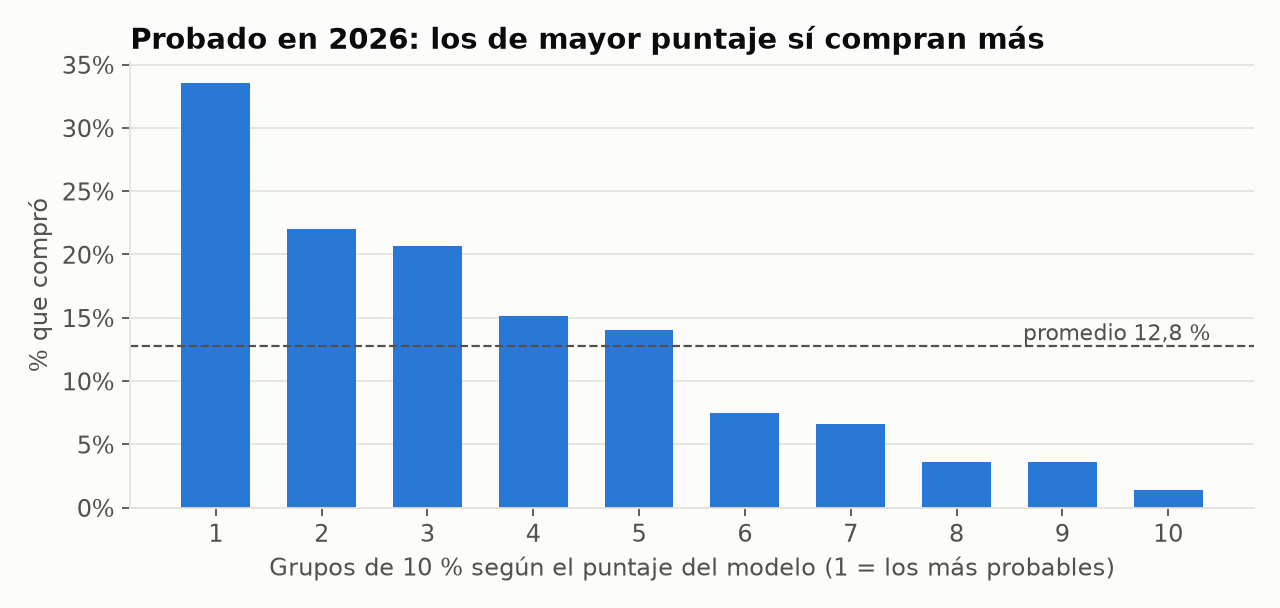
\includegraphics[width=0.82\linewidth]{fig/4_lift_modelo.png}
\caption{Conversión real en 2026 por decil de puntaje del modelo entrenado con 2024--2025.}
\end{figure}

\subsection{Qué aprendió el modelo}

La tabla~\ref{tab:drivers} muestra cómo cambian las chances de compra (probabilidad de comprar sobre
probabilidad de no comprar) con cada factor, manteniendo lo demás constante. Como el \textit{one-hot} conserva
todas las categorías, los coeficientes de una variable categórica solo tienen sentido comparados con una
categoría de referencia; \texttt{salidas/drivers.csv} los reporta así.

\begin{table}[!htbp]
\centering
\caption{Efecto sobre las chances de compra (\texttt{salidas/drivers.csv}).}
\label{tab:drivers}
\begin{tabularx}{\linewidth}{L l r}
\toprule
Factor & Frente a & Efecto \\
\midrule
Puntaje previo una desviación estándar más alto & la media & +82 \% \\
Asistir al webinar (además de estar invitado) & no asistir & +43 \% \\
Botón centrado en el beneficio & botón estándar & +24 \% \\
Página de llegada nueva & página base & +17 \% \\
Material descargable & sin material & +16 \% \\
Pago simplificado & pago estándar & +5 \% \\
Pauta en nivel saturado & nivel medio & $-$49 \% \\
Oferta del producto nuevo & sin oferta & $-$38 \% \\
\bottomrule
\end{tabularx}
\end{table}

El efecto del producto es negativo en conversión, pero cada venta del producto vale más del doble (ticket de
€2.827 frente a €1.064), así que el balance en contribución puede ser positivo. Es justo lo que la simulación
tiene que resolver.

% ================================================================== 5
\section{De la predicción a la decisión}

\subsection{Escenarios contrafactuales}

Tomamos las 10.073 oportunidades de los últimos doce meses y le pedimos al modelo la contribución esperada de
cada una dos veces: tal como ocurrió y con la iniciativa aplicada. La diferencia es la ganancia atribuible a la
iniciativa. La contribución esperada de una oportunidad es su probabilidad de compra por el valor de una venta
de su segmento (utilidad bruta menos el costo fijo de €22), menos el costo de publicidad atribuido.

\begin{itemize}
  \item \textbf{Embudo}: todas las oportunidades ven las cuatro mejoras.
  \item \textbf{Webinars}: se invita a los 3.334 contactos conocidos que no lo fueron, y asiste uno de cada
        cuatro, como en el histórico.
  \item \textbf{Producto}: se ofrece a las 5.858 oportunidades de los tres segmentos donde hay evidencia.
  \item \textbf{Publicidad}: como hubo periodos con gasto alto y saturado, se usa la contribución observada en
        esos regímenes, escalada por el volumen de oportunidades por día de campaña. Duplicar el gasto actual
        (nivel medio) cae entre los niveles alto y saturado.
\end{itemize}

\subsection{Dos capas de incertidumbre}

La primera es la de los datos: repetimos el ajuste del modelo y el cálculo de todos los escenarios en 200
muestras \textit{bootstrap} del histórico. La segunda es la de la ejecución: ninguna iniciativa cuesta ni llega
exactamente a lo planeado, así que en 10.000 simulaciones combinamos una réplica \textit{bootstrap} con costos y
alcances tomados de distribuciones triangulares:

\begin{table}[!htbp]
\centering
\caption{Supuestos de ejecución a doce meses (\texttt{SUPUESTOS} en \texttt{src/bi/model.py}).}
\begin{tabularx}{\linewidth}{l L l}
\toprule
Iniciativa & Costo de implementación (mín. / probable / máx.) & Alcance \\
\midrule
Embudo & €8 mil / €12 mil / €20 mil (diseño, desarrollo y pruebas A/B) & 70--100 \% \\
Webinars & €9,6 mil / €14,4 mil / €24 mil (12 sesiones al año) & 50--100 \% \\
Publicidad & €0 / €2 mil / €5 mil (gestión; la pauta ya está en los datos) & 100 \% \\
Producto & €15 mil / €25 mil / €45 mil (desarrollo y lanzamiento) & 30--90 \% \\
\bottomrule
\end{tabularx}
\end{table}

Estos costos son supuestos nuestros y no salen de los datos. Por eso en la sección~\ref{sec:p6} indicamos cuánto
tendrían que cambiar para que cambie la recomendación.

% ================================================================== 6
\section{Resultados}
\label{sec:resultados}

\subsection{P1. Crecimiento}

La tabla siguiente compara los últimos doce meses (mayo de 2025 a abril de 2026) con los doce
anteriores. Las cifras salen de \texttt{salidas/crecimiento.csv}.

\begin{table}[!htbp]
\centering
\caption{Últimos doce meses frente a los doce anteriores.}
\begin{tabular}{l r r r}
\toprule
Indicador & Año anterior & Último año & Cambio \\
\midrule
Oportunidades & 7.680 & 10.073 & +31 \% \\
Ventas & 694 & 1.224 & +76 \% \\
Conversión & 9,0 \% & 12,2 \% & +3,2 p.p. \\
Costo por venta & €81 & €66 & $-$18 \% \\
Contribución & €487 mil & €934 mil & +92 \% \\
\bottomrule
\end{tabular}
\end{table}

Las ventas crecen más que las oportunidades y la contribución más que las ventas: el crecimiento viene sobre
todo de vender mejor, no de traer más gente. La señal de alerta es que el gasto total en publicidad atribuido
sube 44 \%, y no sabemos si ese costo atribuido recoge todo lo que realmente se pagó.

\begin{figure}[!htbp]
\centering
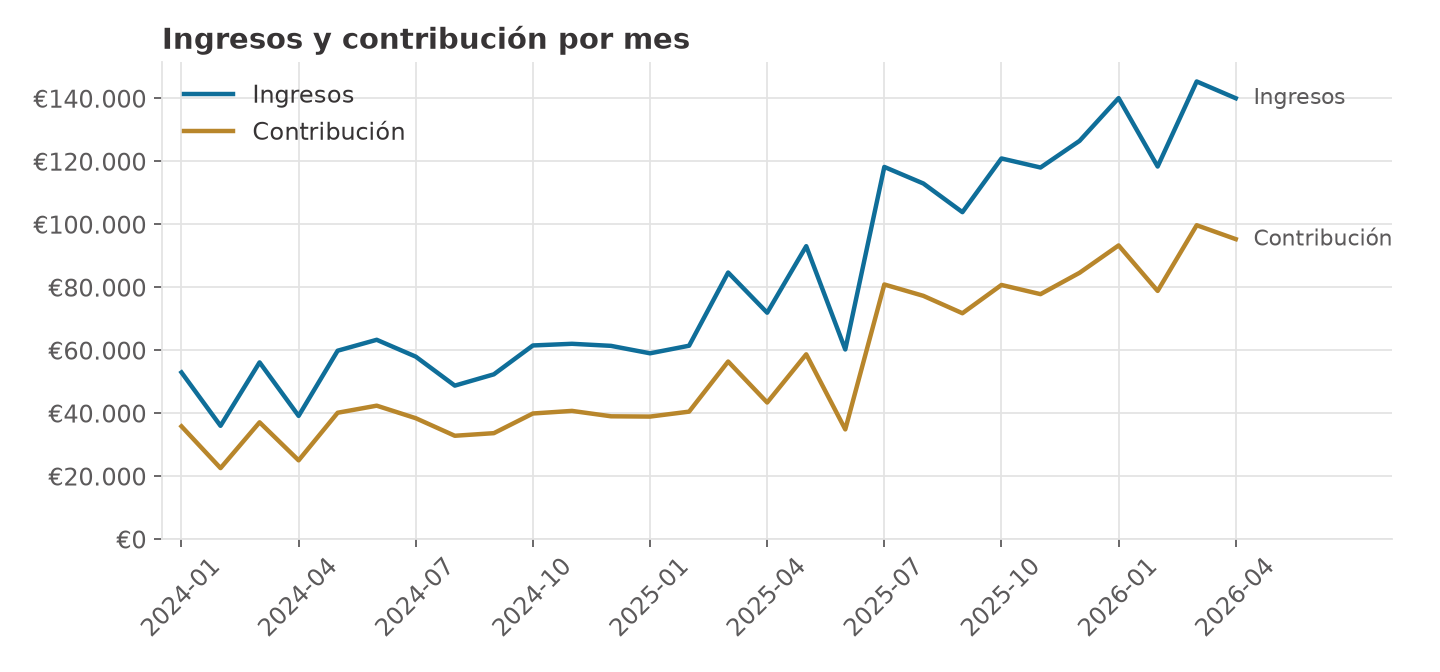
\includegraphics[width=0.85\linewidth]{fig/0_evolucion_mensual.png}
\caption{Ingresos y contribución por mes (vista \texttt{kpi}, dimensión mes).}
\end{figure}

\textbf{Decisión:} el negocio funciona; conviene invertir en lo que hace vender mejor, no en traer más tráfico.

\subsection{P2. Dónde está el valor}

Facebook y Google traen el 39 \% de las oportunidades pero solo el 13 \% de la contribución. Email, SEO y
Webinar, en cambio, traen el 40 \% de las oportunidades y el 69 \% de la contribución. Por segmento, Enterprise
es el 10 \% de las oportunidades y aporta el 24 \% de la contribución. España concentra el 47 \% de los ingresos,
pero la rentabilidad por oportunidad es parecida en todos los países, así que el país no cambia la decisión
(\texttt{salidas/pivote\_ingresos\_region\_segmento.csv}).

\begin{figure}[!htbp]
\centering
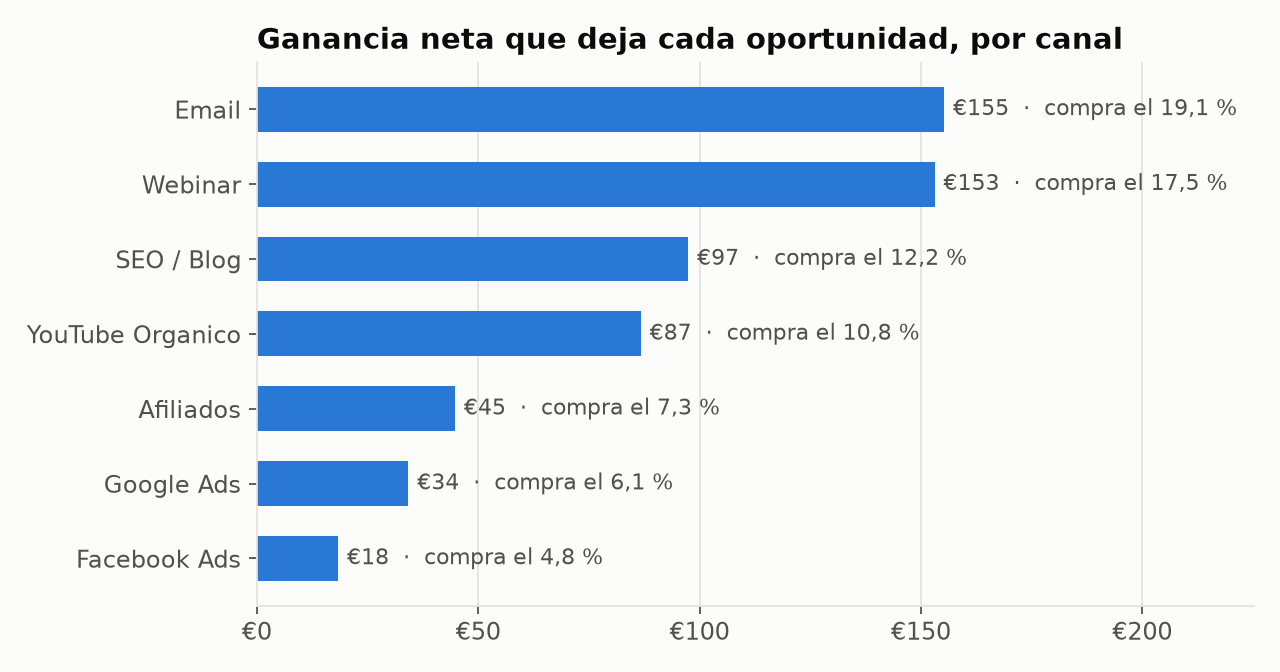
\includegraphics[width=0.8\linewidth]{fig/1_canales.png}
\caption{Contribución por oportunidad y conversión por canal (vista \texttt{kpi}, dimensión canal).}
\end{figure}

\textbf{Decisión:} no poner más dinero en Facebook y Google; el valor está en los canales propios y en Enterprise.

\subsection{P3. Qué explica la mejora}

La conversión pasa de cerca de 9 \% a cerca de 13 \% en el tercer trimestre de 2025, el mismo trimestre en que el
embudo completo empieza a usarse (16 \% de las oportunidades). Dentro de cada trimestre el modelo encuentra que
las oportunidades con las mejoras compran más, lo que apoya la idea de que el embudo tiene un efecto propio.

Pero el dato mensual obliga a ser cautos. En julio de 2025 la conversión ya es de 13,5 \% cuando ninguna
oportunidad tenía todavía el embudo completo; y en el cuarto trimestre la adopción sube a 24 \% mientras la
conversión baja a 11,8 \%. Además, entre junio y julio el costo por venta cae de €160 a €46, lo que sugiere que
terminó un periodo de pauta saturada y cambió la mezcla de canales. Nuestra lectura es que el embudo explica una
parte de la mejora, no toda, y que el salto de julio tiene al menos otra causa que no podemos aislar con estos
datos. Confirmarlo requiere revisar cuándo se activó cada componente por separado y si hubo otros cambios
(precios, equipo comercial) en esas fechas.

\begin{figure}[!htbp]
\centering
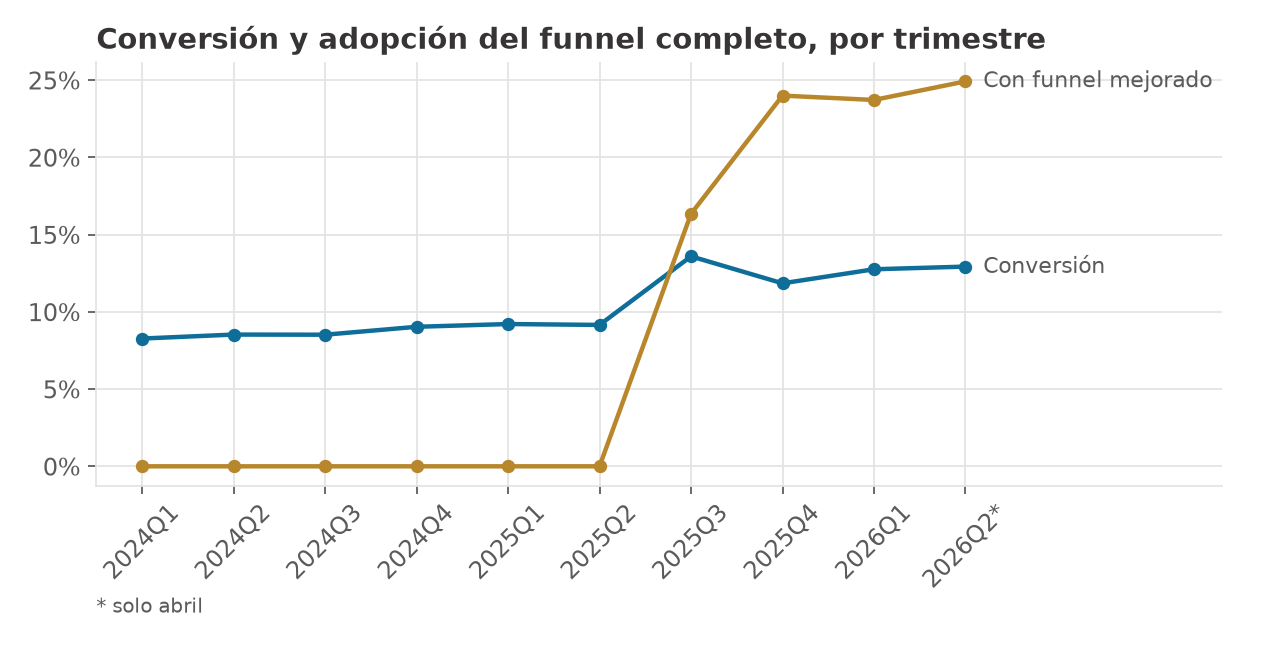
\includegraphics[width=0.8\linewidth]{fig/2_tendencia_funnel.png}
\caption{Conversión y adopción del embudo completo por trimestre (vista \texttt{kpi}, dimensión trimestre).}
\end{figure}

\textbf{Decisión:} extender el embudo, pero con un grupo de control que mida su efecto real.

\subsection{P4. Publicidad}

Pasar del nivel medio de gasto (el vigente) al saturado multiplica el gasto diario por 2,5 pero las
oportunidades solo por 1,3, y además llegan peor calificadas: el puntaje medio baja de 52,5 a 37,8. Cada venta
pasa a costar €853 en vez de €178, y cada oportunidad deja $-$€3 en lugar de €36
(\texttt{salidas/ads\_niveles.csv}).

\begin{figure}[!htbp]
\centering
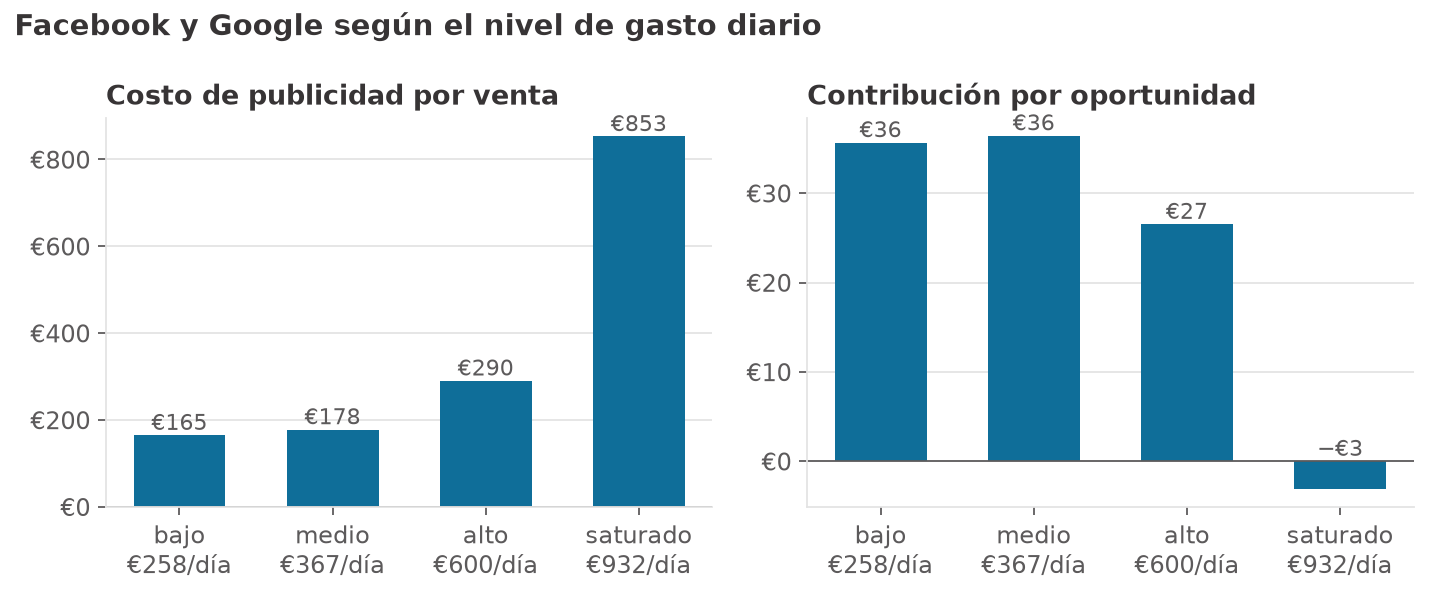
\includegraphics[width=0.9\linewidth]{fig/3_ads_saturacion.png}
\caption{Costo por venta y contribución por oportunidad según el nivel de gasto (vista \texttt{ads\_niveles}).}
\end{figure}

Una salvedad: los niveles de gasto funcionaron como épocas, no como un experimento. El nivel bajo, por ejemplo,
solo existió antes de que llegara el embudo. La dirección del resultado es muy clara, pero su magnitud mezcla el
efecto del gasto con el del momento.

\textbf{Decisión:} no duplicar la publicidad.

\subsection{P5. Qué hace que alguien compre}

El puntaje previo es, de lejos, el factor más fuerte, seguido por la asistencia al webinar y las mejoras del
embudo (tabla~\ref{tab:drivers}). Fuera de muestra, el modelo ordena bien a los interesados, así que además de
servir para comparar iniciativas puede usarse para que el equipo comercial priorice a quién llamar. Para ese uso
conviene reentrenarlo sin la variable de trimestre, que no aporta nada al puntuar periodos futuros, y revisar su
calibración.

\textbf{Decisión:} usar el puntaje para ordenar la atención comercial y, en los webinars, medir asistentes y no invitados.

\subsection{P6. Qué iniciativa conviene}
\label{sec:p6}

\begin{table}[!htbp]
\centering
\caption{Contribución adicional a doce meses en 10.000 simulaciones (\texttt{salidas/montecarlo\_resumen.csv}).}
\begin{tabular}{l r r r r}
\toprule
Iniciativa & Esperado & P10 & P90 & P(pérdida) \\
\midrule
Producto nuevo (3 segmentos) & €175 mil & €75 mil & €285 mil & 0,1 \% \\
Embudo mejorado & €120 mil & €77 mil & €166 mil & 0,0 \% \\
Webinars & €32 mil & €8 mil & €56 mil & 3,9 \% \\
Duplicar publicidad & $-$€101 mil & $-$€158 mil & $-$€45 mil & 99,5 \% \\
\bottomrule
\end{tabular}
\end{table}

\begin{figure}[!htbp]
\centering
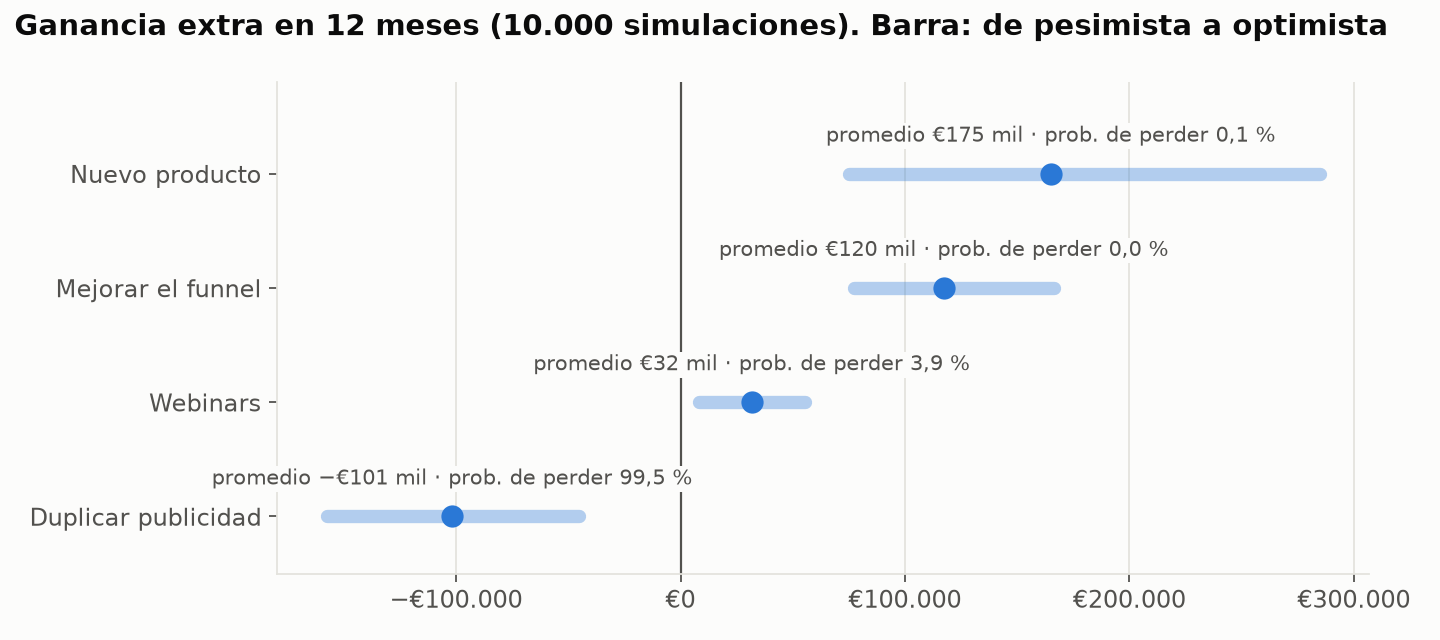
\includegraphics[width=0.9\linewidth]{fig/5_montecarlo.png}
\caption{Valor esperado (punto) y rango entre los percentiles 10 y 90 (barra) por iniciativa.}
\end{figure}

El producto tiene el mayor valor esperado y también el rango más ancho. El embudo deja algo menos, pero con un
rango estrecho y con el mejor retorno por euro invertido (unas nueve veces su costo, frente a seis del producto).
Duplicar la publicidad pierde dinero en prácticamente todas las simulaciones.

Los umbrales que cambiarían la recomendación son dos. Si lanzar el producto costara más de €84 mil, el embudo
pasaría a tener el mayor valor esperado. Y los webinars solo compensan si el programa cuesta menos de €48 mil al
año.

\textbf{Decisión:} embudo ahora, por ser la apuesta más segura; producto en piloto, por ser la más incierta.

% ================================================================== 7
\section{Limitaciones}

Las probabilidades de pérdida de la tabla anterior hay que leerlas con cuidado. Recogen el ruido muestral y la
incertidumbre de ejecución, pero suponen que el modelo está bien especificado. Hay cuatro razones para pensar que
la incertidumbre real es mayor:

\begin{enumerate}
  \item \textbf{El producto se estima con muy poca evidencia.} Se ofreció 554 veces y se vendió 55. El escenario lo
        extiende a casi diez veces más oportunidades y no considera canibalización ni efecto novedad. Su cifra
        debe tomarse como un techo optimista, no como una estimación central.
  \item \textbf{El \textit{bootstrap} remuestrea filas sueltas.} Las palancas cambiaron por épocas, y remuestrear
        fila por fila ignora esa estructura. Un \textit{bootstrap} por bloques mensuales daría rangos más anchos.
  \item \textbf{Los efectos del webinar y del embudo no salen de experimentos.} Quienes asisten a un webinar se
        seleccionan solos, y a los invitados se les eligió con mejor puntaje (62 frente a 56). Es probable que el
        +43 \% de la asistencia sobreestime el efecto real.
  \item \textbf{Las iniciativas se evaluaron por separado.} El embudo sube la conversión y el producto la baja; en
        un modelo logístico esos efectos no se suman. Antes de ejecutar ambas habría que simular el escenario
        combinado.
\end{enumerate}

Por último, los datos son sintéticos. El método se puede reutilizar con datos reales; las cifras no describen
a ninguna empresa.

% ================================================================== 8
\section{Conclusiones y recomendación}

El negocio crece por eficiencia: convierte mejor y gasta menos por venta. La publicidad pagada es la parte menos
rentable de la operación, y llevarla a niveles altos de gasto la vuelve deficitaria. Entre las iniciativas, el
embudo mejorado es la apuesta más segura y el producto nuevo la de mayor potencial, aunque también la menos
respaldada por los datos.

Nuestra recomendación a la gerencia:

\begin{enumerate}
  \item \textbf{Extender el embudo mejorado}, que hoy ve cerca de una de cada cuatro oportunidades. Hacerlo
        dejando un grupo de control al azar, para medir su efecto de forma limpia y no depender solo de la
        comparación histórica.
  \item \textbf{Pilotear el producto nuevo} durante un trimestre en B2B Services, Ecommerce y Enterprise,
        ofreciéndolo a un grupo elegido al azar. Escalarlo solo si el piloto confirma que compensa la menor
        conversión.
  \item \textbf{No duplicar la publicidad.} Mantener el nivel actual y pedir a finanzas el gasto real de pauta,
        que el archivo no trae.
  \item \textbf{Webinars solo si cuestan menos de €48 mil al año}, y medir asistentes, no invitados.
  \item \textbf{Usar el puntaje del modelo} para ordenar la atención comercial.
\end{enumerate}

\newpage
\appendix
\section{Diccionario de variables}
\label{anx:diccionario}

\begin{table}[!htbp]
\centering\small
\begin{tabularx}{\linewidth}{>{\ttfamily}l l L}
\toprule
\normalfont Variable & Tipo & Descripción y uso \\
\midrule
transaction\_id & Identificador & Una oportunidad; se valida que no se repita \\
date & Fecha & Día de la oportunidad \\
month, quarter & Fecha derivada & Mes y trimestre; se valida que coincidan con la fecha \\
channel & Categórica & Canal de llegada (7 valores) \\
campaign\_objective & Categórica & Objetivo de la campaña (captación, nutrición, recuperación\ldots) \\
customer\_segment & Categórica & B2B Services, Enterprise, Ecommerce, Creator, SMB \\
lifecycle\_stage & Categórica & Visitante nuevo, contacto conocido o cliente recurrente \\
device, geo\_region & Categórica & Dispositivo y país \\
ad\_budget\_level & Ordinal & Nivel de gasto en pauta (bajo a saturado); solo canales pagados \\
campaign\_daily\_spend\_eur & Numérica & Gasto diario de la campaña; varía por fila y no es aditivo \\
cost\_attributed\_eur & Numérica & Costo de pauta atribuido; entra en la contribución, no en el modelo \\
landing\_variant, cta\_variant & Categórica & Variantes de página y botón (palancas del embudo) \\
lead\_magnet, checkout\_simplified & Binaria & Material descargable y pago simplificado \\
webinar\_invited, webinar\_attended & Binaria & Invitación y asistencia al webinar \\
new\_product\_offer & Binaria & Se ofreció el producto nuevo \\
lead\_score & Numérica (1--99) & Puntaje previo del interesado; la variable más predictiva \\
converted\_to\_sale & Binaria & Compró; variable objetivo \\
days\_to\_close & Numérica & Días hasta la compra; solo si compró; excluida (fuga) \\
aov\_eur, revenue\_eur & Numérica & Ticket e ingreso; 0 si no compró \\
gross\_margin\_pct, gross\_profit\_eur & Numérica & Margen y utilidad bruta; excluidas del modelo \\
contribution\_profit\_eur & Numérica & Contribución; medida de valor del informe \\
\bottomrule
\end{tabularx}
\end{table}

\section{Reproducción}

\begin{lstlisting}[language=bash, backgroundcolor=\color{udfondo}]
make install       # entorno con uv
make test          # pruebas automáticas
make run           # valida, calcula, entrena, simula y regenera salidas y figuras
make pdf           # compila este informe y la presentación (tectonic)
\end{lstlisting}

El archivo original debe estar en \texttt{data/original/dataset\_ventas\_transaccional\_sintetico\_es.csv}.

\section{Código SQL}

\subsection*{\texttt{sql/01\_preparacion.sql}}
\lstinputlisting{../sql/01_preparacion.sql}
\subsection*{\texttt{sql/02\_indicadores.sql}}
\lstinputlisting{../sql/02_indicadores.sql}
\subsection*{\texttt{sql/03\_modelo\_dimensional.sql}}
\lstinputlisting{../sql/03_modelo_dimensional.sql}

\end{document}
